%%%%%%%%%%%%%%%%%%%%%%%%%%%%%%%%%%%%

\section{6.3. Teste qui-quadrado de \textit{Goodness of fit}}

%%%%%%%%%%%%%%%%%%%%%%%%%%%%%%%%%%%

\subsection{Dados de Weldon}

%%%%%%%%%%%%%%%%%%%%%%%%%%%%%%%%%%%

\begin{frame}
\frametitle{Dados de Weldon}

\twocol{0.7}{0.3}
{
\begin{itemize}
\justifying
\small
\item Walter Frank Raphael Weldon (1860 - 1906), foi um biólogo inglês evolucionário e um dos fundadores da biometria. Além disso, ele foi o editor fundador da revista \textit{Biometrika}, com Francis Galton e Karl Pearson.
\justifying
\item Em 1894, ele jogou 12 dados 26.306 vezes e registrou a quatidade de vezes que sairam os número 5 e 6 (que ele considerou como sucesso).

\end{itemize}
}
{
\begin{center}
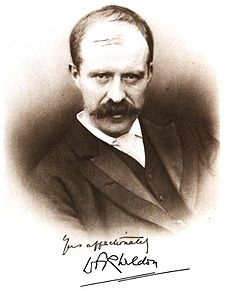
\includegraphics[width=\textwidth]{6-3_chisq_gof/weldon.jpeg}
\end{center}
}
\begin{itemize}
\justifying
\small
\item Observou-se que os números 5 ou 6 ocorreram com mais frequência do que o esperado, e Pearson levantou a hipótese de que isso ocorreu provavelmente devido à construção dos dados. Os dados mais baratos têm pips (aqueles pontinhos pretos) ocos e, como os lados opostos aumentam para 7, a face com 6 pips é mais leve do que a face oposta, que tem apenas 1 pip.

\end{itemize}

\end{frame}

%%%%%%%%%%%%%%%%%%%%%%%%%%%%%%%%%%%

\begin{frame}
\frametitle{Dados de Labby}
\scalefont{0.8}
\twocol{0.5}{0.5}
{
\begin{itemize}
\justifying
\item Em 2009, Zacariah Labby (U de Chicago), repetiu o experimento de Weldon usando uma máquina de contagem de lançadores de dados caseiros.
\begin{center}
\justifying
\webURL{http://www.youtube.com/watch?v=95EErdouO2w}
\end{center}
\justifying
\item O processo de criação de imagens demorava cerca de 20 segundos por rolagem.

\end{itemize}
}
{
\begin{center}
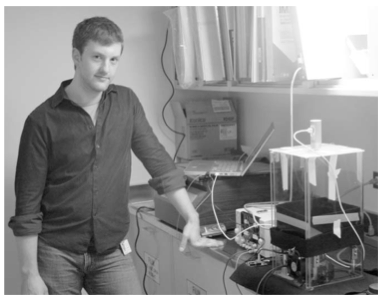
\includegraphics[width=\textwidth]{6-3_chisq_gof/labby.png}
\end{center}
}

\begin{itemize}
\justifying
\item Cada dia havia $\sim$ 150 imagens para processar manualmente.
\justifying
\item Nesse ritmo, a experiência de Weldon foi repetida em pouco mais de seis dias inteiros.
\justifying
\item Leitura recomendada:\webURL{http://galton.uchicago.edu/about/docs/labby09dice.pdf}

\end{itemize}

\end{frame}

%%%%%%%%%%%%%%%%%%%%%%%%%%%%%%%%%%%

\begin{frame}
\frametitle{Dados de Labby (cont.)}

\begin{itemize}
\justifying
\item Labby não observou o mesmo fenômeno que Weldon (maior frequência dos números de 5 e 6).
\justifying
\item A automação permitiu que Labby coletasse mais dados do que Weldon em 1894, e, em vez de registrar "sucessos" e "falhas", Labby registrava o número individual de pips em cada dado.

\end{itemize}

\begin{center}
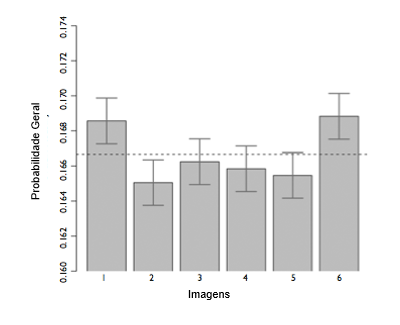
\includegraphics[width=0.5\textwidth]{6-3_chisq_gof/labbyPipCounts.png}
\end{center}

\end{frame}

%%%%%%%%%%%%%%%%%%%%%%%%%%%%%%%%%%%

\subsection*{Criando uma estatística de teste para tabelas unidirecionais}

%%%%%%%%%%%%%%%%%%%%%%%%%%%%%%%%%%%

\begin{frame}
\frametitle{Contagens esperadas}
\justifying
\pq{Labby rolou 12 dados 26.306 vezes. Se cada lado tiver a mesma probabilidade de aparecer, quantos 1s, 2s, $\cdots$, 6s ele esperaria observar?}

\begin{enumerate}[(a)]
\item $\frac{1}{6}$
\item $\frac{12}{6}$
\item $\frac{26,306}{6}$
\solnMult{ $\frac{12 \times 26,306}{6}$ } \soln{\only<2>{\orange{$= 52,612$}}}
\end{enumerate}

\end{frame}

%%%%%%%%%%%%%%%%%%%%%%%%%%%%%%%%%%%

\begin{frame}
\frametitle{Sumarizando os resultados de Labby}
\justifying
A tabela abaixo mostra as contagens observadas e esperadas da experiência de Labby.

{
\begin{center}
\renewcommand\arraystretch{1.25}
\scalefont{0.7}
\begin{tabular}{c | c c}
Resultado	& Observado	& Esperado \\
\hline
1		& 53,222		& 52,612 \\
2		& 52,118		& 52,612 \\
3		& 52,465		& 52,612 \\
4		& 52,338		& 52,612 \\
5		& 52,244		& 52,612 \\
6		& 53,285		& 52,612 \\
\hline
Total		& 315,672		& 315,672
\end{tabular}
\end{center}
}

\pause
\small{\justifying
\dq{Por que, para todos os resultados, as contagens esperadas são as mesmas mas as contagens observadas são diferentes? À primeira vista, parece haver uma inconsistência entre as contagens observadas e esperadas?}
}
\end{frame}

%%%%%%%%%%%%%%%%%%%%%%%%%%%%%%%%%%%

\begin{frame}
\frametitle{Definindo as hipóteses}
\justifying
\dq{Esses dados fornecem evidências convincentes de uma inconsistência entre as contagens observadas e esperadas?}

\pause

\begin{itemize}
\justifying
\item[$H_0$:] Não há inconsistência entre as contagens observadas e as esperadas. \hlGr{As contagens observadas seguem a mesma distribuição que as contagens esperadas.}

\pause
\justifying
\item[$H_A$:] Existe uma inconsistência entre as contagens observadas e as esperadas. \hlGr{As contagens observadas \orange {não} seguem a mesma distribuição das contagens esperadas.} Existe um viés para que um lado apareça mais vezes no lançamento de um dado.
\end{itemize}

\end{frame}

%%%%%%%%%%%%%%%%%%%%%%%%%%%%%%%%%%%

\begin{frame}
\frametitle{Avaliando as hipóteses}

\begin{itemize}
\justifying
\item Para avaliar essas hipóteses, quantificamos quão diferentes são as contagens observadas das contagens esperadas.

\pause
\justifying
\item Grandes desvios do que seria esperado com base na variação amostral por si só fornecem fortes evidências para a hipótese alternativa.

\pause
\justifying
\item Isso é chamado de teste de \hl{goodness of fit}, ou \textit{qualidade de ajuste}, pois estamos avaliando o quão bem os dados observados se ajustam à distribuição esperada.

\end{itemize}

\end{frame}

%%%%%%%%%%%%%%%%%%%%%%%%%%%%%%%%%%%

\subsection{A estatística do teste do qui-quadrado}

%%%%%%%%%%%%%%%%%%%%%%%%%%%%%%%%%%%

\begin{frame}
\frametitle{Anatomia de uma estatística de teste}

\begin{itemize}
\justifying
\item A forma geral de uma estatística de teste é
\[ \frac{\text{estimativa pontual} - \text{valor nulo}}{\text{erro padrão da estimativa pontual}} \]

\pause
\justifying
\item Esta construção é baseada em 
\begin{enumerate}
\justifying
\item identificar a diferença entre uma estimativa pontual e um valor esperado, supondo que a hipótese nula é verdadeira, e
\justifying
\item padronizar essa diferença usando o erro padrão da estimativa pontual. 
\end{enumerate}
\pause
\justifying
Essas duas ideias ajudarão na construção de uma estatística de teste apropriada para dados de contagem.

\end{itemize}

\end{frame}

%%%%%%%%%%%%%%%%%%%%%%%%%%%%%%%%%%%

\begin{frame}
\frametitle{Estatística qui-quadrado}
\justifying
Ao lidar com contagens e investigar quão longe as contagens observadas estão das contagens esperadas, usamos uma nova estatística de teste chamada \hl{estatística de qui-quadrado ($ \chi^2 $)}.

$\:$ \\

\pause

\formula{Estatística de $\chi^2$ }
{
\[\chi^2 = \sum_{i = 1}^k \frac{(O - E)^2}{E} \qquad \text{onde $k$ = número total de células} \]
}

\end{frame}

%%%%%%%%%%%%%%%%%%%%%%%%%%%%%%%%%%%

\begin{frame}
\frametitle{Calculando a estatística do qui-quadrado}

\begin{center}
\renewcommand\arraystretch{1.8}
\begin{tabular}{c | c c | c}
Resultado	& Observado	& Esperado 	& $\frac{(O - E)^2}{E}$\\
\hline
1		& 53,222		& 52,612 		& $\frac{(53,222 - 52,612)^2}{52,612} = 7.07$ \\
\pause
2		& 52,118		& 52,612 		& $\frac{(52,118 - 52,612)^2}{52,612} = 4.64$ \\
\pause
3		& 52,465		& 52,612 		& $\frac{(52,465 - 52,612)^2}{52,612} = 0.41$ \\
\pause
4		& 52,338		& 52,612 		& $\frac{(52,338 - 52,612)^2}{52,612} = 1.43$\\
\pause
5		& 52,244		& 52,612 		& $\frac{(52,244 - 52,612)^2}{52,612} = 2.57$\\
\pause
6		& 53,285		& 52,612 		& $\frac{(53,285 - 52,612)^2}{52,612} = 8.61$\ \\
\hline
\pause
Total		& 315,672		& 315,672		& 24.73
\end{tabular}
\end{center}

\end{frame}

%%%%%%%%%%%%%%%%%%%%%%%%%%%%%%%%%%%

\begin{frame}
\frametitle{Por que qui-\underline{quadrado}?}

\justifying
Tomar o quadrado da diferença entre o resultado observado e o esperado permite duas coisas duas coisas:
\pause
\begin{itemize}
\justifying
\item Qualquer diferença padronizada que seja quadrada será agora positiva.
\pause
\justifying
\item Diferenças que já pareciam incomuns se tornarão muito maiores depois de se tomar o quadrado.
\end{itemize}

\vspace{1cm}

\pause
\justifying
\dq{Quando já vimos isso antes?}

\end{frame}

%%%%%%%%%%%%%%%%%%%%%%%%%%%%%%%%%%%

\subsection{A distribuição de qui-quadrado e áreas de descoberta}

%%%%%%%%%%%%%%%%%%%%%%%%%%%%%%%%%%%

\begin{frame}
\frametitle{A distribuição de qui-quadrado}

\begin{itemize}
\justifying
\item Para determinar se a estatística $\chi^2$ que calculamos é considerada excepcionalmente alta ou não, precisamos primeiro descrever sua distribuição.

\pause
\justifying
\item A distribuição qui-quadrado tem apenas um parâmetro chamado \hl {graus de liberdade (df)}, que influencia a forma, o centro e a largura da distribuição. \\

\end{itemize}

\pause

$\:$ \\
\justifying
\scalefont{0.8}
Lembre-se que até agora, vimos três outras distribuições contínuas:
\begin{itemize}
\justifying
\item[-] Distribuição normal: unimodal e simétrica com dois parâmetros (média e desvio padrão).
\justifying
\item[-] Distribuição T: unimodal e simétrica com um parâmetro (graus de liberdade).
\justifying
\item[-] Distribuição F: unimodal e inclinada à direita com dois parâmetros (graus de liberdade ou numerador, que é a variância entre grupos, e denominador, que é a varição dentro do grupo).
\end{itemize}


\end{frame}

%%%%%%%%%%%%%%%%%%%%%%%%%%%%%%%%%%%

\begin{frame}
\footnotesize
\frametitle{Prática}
\justifying
\pq{Qual das seguintes afirmações é falsa?}

\begin{center}
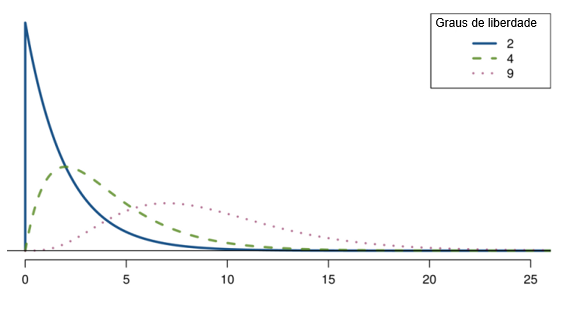
\includegraphics[width=0.7\textwidth]{6-3_chisq_gof/chiSquareDistributionWithInceasingDF.png}
\end{center}

À medida que df aumenta,
\begin{enumerate}[(a)]
\justifying
\item o centro da distribuição $\chi^2$ aumenta também.
\justifying
\item a variabilidade da distribuição $\chi^2$ aumenta também.
\justifying
\solnMult{a forma da distribuição $\chi^2$ torna-se mais assimétrica (menos parecida com uma normal).}
\end{enumerate}

\end{frame}

%%%%%%%%%%%%%%%%%%%%%%%%%%%%%%%%%%%

\begin{frame}[fragile]
\frametitle{Encontrando a área sob a curva da distribuição qui-quadrado}

\begin{itemize}
\justifying
\item P-valor = área da cauda sob a distribuição qui-quadrado.

\pause
\justifying
\item Para isso, podemos usar uma linguagem de programação, ou uma \hl{tabela de probabilidades qui-quadrado}.

\pause
\justifying
\item  Esta tabela funciona como a tabela $t$, mas fornece apenas os valores de cauda superiores.
\end{itemize}

\begin{center}
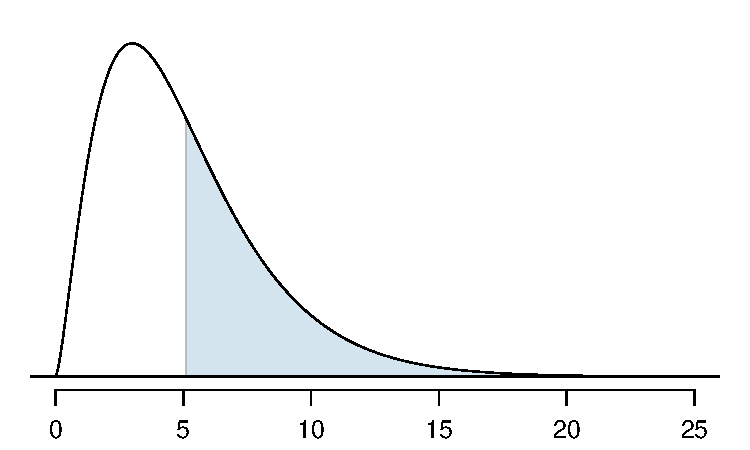
\includegraphics[width=0.6\textwidth]{6-3_chisq_gof/above5Point1WithDF5.pdf}
\end{center}

\end{frame}
%%%%%%%%%%%%%%%%%%%%%%%%%%%%%%%%%%%

\begin{frame}[fragile]
\frametitle{Encontrando a área sob a curva da distribuição qui-quadrado}

{\scriptsize
\begin{center}
\begin{tabular}{r | rrrr | rrrr |}
  \hline
Cauda superior & 0.3 & 0.2 & 0.1 & 0.05 & 0.02 & 0.01 & 0.005 & 0.001 \\ 
  \hline
df \hfill 1 &  1.07 &  1.64 &  2.71 &  3.84 &  5.41 &  6.63 &  7.88 &  10.83 \\ 
  2 &  2.41 &  3.22 &  4.61 &  5.99 &  7.82 &  9.21 &  10.60 &  13.82 \\ 
  3 &  3.66 &  4.64 &  6.25 &  7.81 &  9.84 &  11.34 &  12.84 &  16.27 \\ 
  4 &  4.88 &  5.99 &  7.78 &  9.49 &  11.67 &  13.28 &  14.86 &  18.47 \\ 
  5 &  6.06 &  7.29 &  9.24 &  11.07 &  13.39 &  15.09 &  16.75 &  20.52 \\ 
  \hline
  6 &  7.23 &  8.56 &  10.64 &  12.59 &  15.03 &  16.81 &  18.55 &  22.46 \\ 
  7 &  8.38 &  9.80 &  12.02 &  14.07 &  16.62 &  18.48 &  20.28 &  24.32 \\ 
  $\cdots$ &   &   &   &   &   &   &   &   \\ 
\end{tabular}
\end{center}
}

\end{frame}

%%%%%%%%%%%%%%%%%%%%%%%%%%%%%%%%%%%

\begin{frame}
\frametitle{Encontrando a área sob a curva da distribuição qui-quadrado}
\justifying
\dq{Estimar a área sombreada sob a curva da distribuição qui-quadrado com $df = 6$.}

\twocol{0.6}{0.4}{
\begin{center}
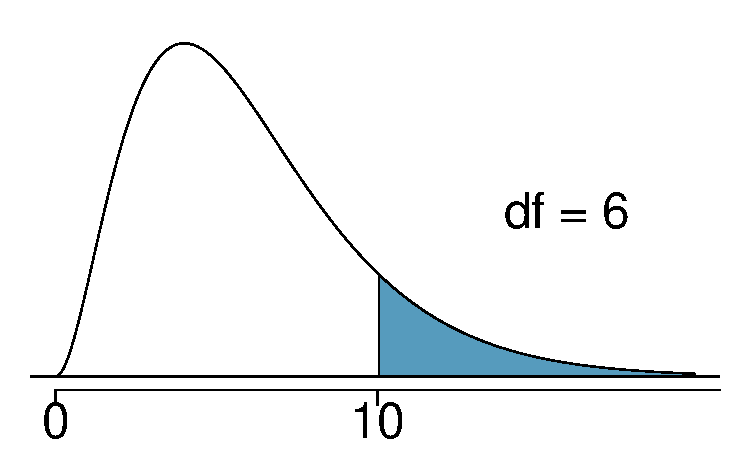
\includegraphics[width=0.67\textwidth]{6-3_chisq_gof/above10WithDF6.pdf}
\end{center}
}
{\only<2 |handout:0>{\orange{$P(\chi^2_{df = 6} > 10)$\\ está entre 0.1 e 0.2}}
}
\end{frame}
%%%%%%%%%%%%%%%%%%%%%%%%%%%%%%%%%%%

\begin{frame}
\frametitle{Encontrando a área sob a curva da distribuição qui-quadrado}

\only<1>{
\begin{center}
{\footnotesize
\begin{tabular}{r | rrrr | rrrr |}
  \hline
Cauda superior & 0.3 & 0.2 & 0.1 & 0.05 & 0.02 & 0.01 & 0.005 & 0.001 \\ 
  \hline
df \hfill 1 &  1.07 &  1.64 &  2.71 &  3.84 &  5.41 &  6.63 &  7.88 &  10.83 \\ 
  2 &  2.41 &  3.22 &  4.61 &  5.99 &  7.82 &  9.21 &  10.60 &  13.82 \\ 
  3 &  3.66 &  4.64 &  6.25 &  7.81 &  9.84 &  11.34 &  12.84 &  16.27 \\ 
  4 &  4.88 &  5.99 &  7.78 &  9.49 &  11.67 &  13.28 &  14.86 &  18.47 \\ 
  5 &  6.06 &  7.29 &  9.24 &  11.07 &  13.39 &  15.09 &  16.75 &  20.52 \\ 
  \hline
  6 &  7.23 &  8.56 &   10.64  &  12.59 &  15.03 &  16.81 &  18.55 &  22.46 \\ 
  7 &  8.38 &  9.80 &  12.02 &  14.07 &  16.62 &  18.48 &  20.28 &  24.32 \\ 
  \hline
\end{tabular}
}
\end{center}
}

\only<2 | handout:0>{
\begin{center}
{\footnotesize
\begin{tabular}{r | rrrr | rrrr |}
  \hline
Cauda superior & 0.3 & 0.2 & 0.1 & 0.05 & 0.02 & 0.01 & 0.005 & 0.001 \\ 
  \hline
df \hfill 1 &  1.07 &  1.64 &  2.71 &  3.84 &  5.41 &  6.63 &  7.88 &  10.83 \\ 
  2 &  2.41 &  3.22 &  4.61 &  5.99 &  7.82 &  9.21 &  10.60 &  13.82 \\ 
  3 &  3.66 &  4.64 &  6.25 &  7.81 &  9.84 &  11.34 &  12.84 &  16.27 \\ 
  4 &  4.88 &  5.99 &  7.78 &  9.49 &  11.67 &  13.28 &  14.86 &  18.47 \\ 
  5 &  6.06 &  7.29 &  9.24 &  11.07 &  13.39 &  15.09 &  16.75 &  20.52 \\ 
  \hline
\rowcolor[gray]{.6}
  6 &  7.23 &  8.56 &   10.64  &  12.59 &  15.03 &  16.81 &  18.55 &  22.46 \\ 
  7 &  8.38 &  9.80 &  12.02 &  14.07 &  16.62 &  18.48 &  20.28 &  24.32 \\ 
  \hline
\end{tabular}
}
\end{center}
}

\only<3 | handout:0>{
\begin{center}
{\footnotesize
\begin{tabular}{r | rrrr | rrrr |}
  \hline
Cauda superior & 0.3 & 0.2 & 0.1 & 0.05 & 0.02 & 0.01 & 0.005 & 0.001 \\ 
  \hline
df \hfill 1 &  1.07 &  1.64 &  2.71 &  3.84 &  5.41 &  6.63 &  7.88 &  10.83 \\ 
  2 &  2.41 &  3.22 &  4.61 &  5.99 &  7.82 &  9.21 &  10.60 &  13.82 \\ 
  3 &  3.66 &  4.64 &  6.25 &  7.81 &  9.84 &  11.34 &  12.84 &  16.27 \\ 
  4 &  4.88 &  5.99 &  7.78 &  9.49 &  11.67 &  13.28 &  14.86 &  18.47 \\ 
  5 &  6.06 &  7.29 &  9.24 &  11.07 &  13.39 &  15.09 &  16.75 &  20.52 \\ 
  \hline
  \rowcolor[gray]{.6}
  6 &  7.23 & \orange{ 8.56 }&  \orange{ 10.64 } &  12.59 &  15.03 &  16.81 &  18.55 &  22.46 \\ 
  7 &  8.38 &  9.80 &  12.02 &  14.07 &  16.62 &  18.48 &  20.28 &  24.32 \\ 
  \hline
\end{tabular}
}
\end{center}
}

\only<4 | handout:0>{
\begin{center}
{\footnotesize
\begin{tabular}{r | r >{\columncolor[gray]{0.6}[.5\tabcolsep]}r >{\columncolor[gray]{0.6}[.5\tabcolsep]}rr | rrrr |}
  \hline
Cauda superior & 0.3 & \orange{0.2} & \orange{0.1} & 0.05 & 0.02 & 0.01 & 0.005 & 0.001 \\ 
  \hline
df \hfill 1 &  1.07 &  1.64 &  2.71 &  3.84 &  5.41 &  6.63 &  7.88 &  10.83 \\ 
  2 &  2.41 &  3.22 &  4.61 &  5.99 &  7.82 &  9.21 &  10.60 &  13.82 \\ 
  3 &  3.66 &  4.64 &  6.25 &  7.81 &  9.84 &  11.34 &  12.84 &  16.27 \\ 
  4 &  4.88 &  5.99 &  7.78 &  9.49 &  11.67 &  13.28 &  14.86 &  18.47 \\ 
  5 &  6.06 &  7.29 &  9.24 &  11.07 &  13.39 &  15.09 &  16.75 &  20.52 \\ 
  \hline
  \rowcolor[gray]{.6}
  6 &  7.23 & \orange{ 8.56 }&  \orange{ 10.64 } &  12.59 &  15.03 &  16.81 &  18.55 &  22.46 \\ 
  7 &  8.38 &  9.80 &  12.02 &  14.07 &  16.62 &  18.48 &  20.28 &  24.32 \\ 
  \hline
\end{tabular}
}
\end{center}
}

\end{frame}

%%%%%%%%%%%%%%%%%%%%%%%%%%%%%%%%%%%

\begin{frame}
\frametitle{Encontrando a área sob a curva da distribuição qui-quadrado}
\justifying
\pq{Estime a área sombreada (acima de 17) sob a curva $ \chi ^ 2 $ com $df = 9$.}

\twocol{0.6}{0.4}{
\begin{center}
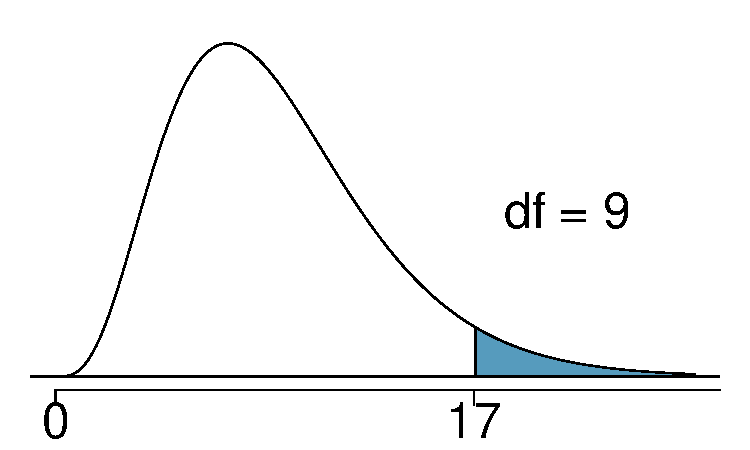
\includegraphics[width=0.67\textwidth]{6-3_chisq_gof/above17WithDF9.pdf}
\end{center}
}
{
{\small
\begin{enumerate}[(a)]
\setlength{\itemsep}{0in}
\item 0.05
\item 0.02
\solnMult{entre 0.02 e 0.05}
\item entre 0.05 e 0.1
\item entre 0.01 e 0.02
\end{enumerate}
}
}
\end{frame}
%%%%%%%%%%%%%%%%%%%%%%%%%%%%%%%%%%%

\begin{frame}
\frametitle{Encontrando a área sob a curva da distribuição qui-quadrado}

\only<1>{
\begin{center}
{\scriptsize
\begin{tabular}{r | rrrr | rrrr |}
  \hline
Cauda superior & 0.3 & 0.2 & 0.1 & 0.05 & 0.02 & 0.01 & 0.005 & 0.001 \\ 
  \hline
df  \hfill 7 &  8.38 &  9.80 &  12.02 &  14.07 &  16.62 &  18.48 &  20.28 &  24.32 \\ 
  8 &  9.52 &  11.03 &  13.36 &  15.51 &  18.17 &  20.09 &  21.95 &  26.12 \\ 
  9 &  10.66 &  12.24 &  14.68 &  16.92 &  19.68 &  21.67 &  23.59 &  27.88 \\ 
  10 &  11.78 &  13.44 &  15.99 &  18.31 &  21.16 &  23.21 &  25.19 &  29.59 \\ 
  \hline
  11 &   12.90 &  14.63 &  17.28 &  19.68 &  22.62 &  24.72 &  26.76 &  31.26 \\ 
\end{tabular}
}
\end{center}
}

\only<2 | handout:0>{
\begin{center}
{\scriptsize
\begin{tabular}{r | rrr >{\columncolor[gray]{0.6}[.5\tabcolsep]}r | >{\columncolor[gray]{0.6}[.5\tabcolsep]}rrrr |}
  \hline
Cauda superior & 0.3 & 0.2 & 0.1 & \orange{ 0.05 } & \orange{ 0.02 } & 0.01 & 0.005 & 0.001 \\ 
  \hline
df  \hfill 7 &  8.38 &  9.80 &  12.02 &  14.07 &  16.62 &  18.48 &  20.28 &  24.32 \\ 
  8 &  9.52 &  11.03 &  13.36 &  15.51 &  18.17 &  20.09 &  21.95 &  26.12 \\ 
    \rowcolor[gray]{.6}
  9 &  10.66 &  12.24 &  14.68 &  \orange{16.92 }&  \orange{19.68} &  21.67 &  23.59 &  27.88 \\ 
  10 &  11.78 &  13.44 &  15.99 &  18.31 &  21.16 &  23.21 &  25.19 &  29.59 \\ 
  \hline
  11 &   12.90 &  14.63 &  17.28 &  19.68 &  22.62 &  24.72 &  26.76 &  31.26 \\ 
  \hline
\end{tabular}
}
\end{center}
}

\end{frame}

%%%%%%%%%%%%%%%%%%%%%%%%%%%%%%%%%%%

\begin{frame}
\frametitle{Encontrando a área sob a curva da distribuição qui-quadrado}
\justifying
\pq{Estime a área sombreada (acima de 30) sob a curva $ \chi ^ 2 $ com $df = 10$.}

\twocol{0.6}{0.4}{
\begin{center}
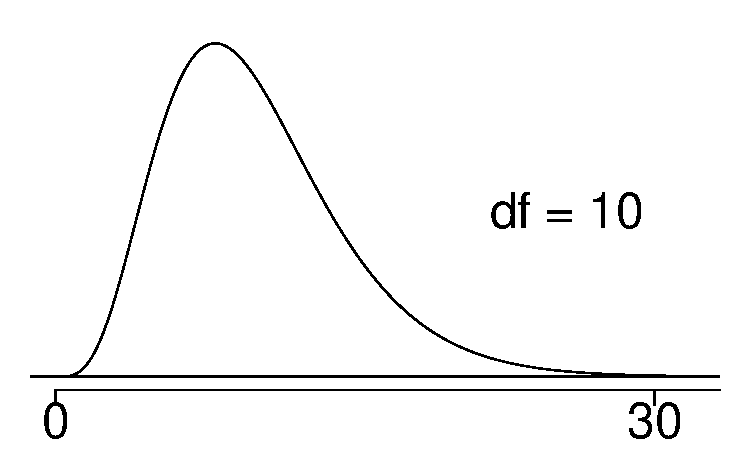
\includegraphics[width=0.67\textwidth]{6-3_chisq_gof/above30WithDF10.pdf}
\end{center}
}
{
{\small
\begin{enumerate}[(a)]
\setlength{\itemsep}{0in}
\item maior que 0.3
\item entre 0.005 e 0.001
\solnMult{menor que 0.001}
\item maior que 0.001
\item não posso dizer usando esta tabela
\end{enumerate}
}
}
\end{frame}
%%%%%%%%%%%%%%%%%%%%%%%%%%%%%%%%%%%

\begin{frame}
\frametitle{Encontrando a área sob a curva da distribuição qui-quadrado}

\only<1>{
\begin{center}
{\scriptsize
\begin{tabular}{r | rrrr | rrrr |}
  \hline
Cauda superior & 0.3 & 0.2 & 0.1 & 0.05 & 0.02 & 0.01 & 0.005 & 0.001 \\ 
  \hline
df  \hfill 7 &  8.38 &  9.80 &  12.02 &  14.07 &  16.62 &  18.48 &  20.28 &  24.32 \\ 
  8 &  9.52 &  11.03 &  13.36 &  15.51 &  18.17 &  20.09 &  21.95 &  26.12 \\ 
  9 &  10.66 &  12.24 &  14.68 &  16.92 &  19.68 &  21.67 &  23.59 &  27.88 \\ 
  10 &  11.78 &  13.44 &  15.99 &  18.31 &  21.16 &  23.21 &  25.19 &  29.59 \\ 
  \hline
  11 &   12.90 &  14.63 &  17.28 &  19.68 &  22.62 &  24.72 &  26.76 &  31.26 \\ 
\end{tabular}
}
\end{center}
}

\only<2 | handout:0>{
\begin{center}
{\scriptsize
\begin{tabular}{r | rrrr | rrr>{\columncolor[gray]{0.6}[.5\tabcolsep]}r | c}
  \cline{1-9}
Cauda superior & 0.3 & 0.2 & 0.1 & 0.05 &  0.02  & 0.01 & 0.005 & \orange{0.001} & \mathhl{\rightarrow}  \\ 
  \cline{1-9}
df  \hfill 7 &  8.38 &  9.80 &  12.02 &  14.07 &  16.62 &  18.48 &  20.28 &  24.32 \\ 
  8 &  9.52 &  11.03 &  13.36 &  15.51 &  18.17 &  20.09 &  21.95 &  26.12 \\ 
  9 &  10.66 &  12.24 &  14.68 &  16.92 &  19.68 &  21.67 &  23.59 &  27.88 \\ 
    \rowcolor[gray]{.6}
  10 &  11.78 &  13.44 &  15.99 &  18.31 &  21.16 &  23.21 &  25.19 &  \orange{29.59} & \mathhl{\rightarrow} \\ 
  \cline{1-9}
  11 &   12.90 &  14.63 &  17.28 &  19.68 &  22.62 &  24.72 &  26.76 &  31.26 \\ 
  \cline{1-9}
\end{tabular}
}
\end{center}
}

\end{frame}

%%%%%%%%%%%%%%%%%%%%%%%%%%%%%%%%%%%

\begin{frame}[fragile]
\frametitle{Encontrando a área sob a curva da distribuição qui-quadrado usando computação}

\begin{itemize}
\justifying
\item Embora as tabelas de probabilidades sejam muito úteis para entender como as distribuições de probabilidade funcionam e fornecer uma referência rápida quando os recursos computacionais não estão disponíveis, elas são um pouco arcaicas.

\pause

\item Usando R:
{\footnotesize
\begin{lstlisting}
pchisq(q = 30, df = 10, lower.tail = FALSE)
# 0.0008566412
\end{lstlisting}
}

\pause

\item Usando um applet da web:

\webURL{http://bitly.com/dist_calc}

\end{itemize}

\end{frame}

%%%%%%%%%%%%%%%%%%%%%%%%%%%%%%%%%%%

\subsection{Encontrar o p-valor de um teste do qui-quadrado}

%%%%%%%%%%%%%%%%%%%%%%%%%%%%%%%%%%%

\begin{frame}
\frametitle{De volta aos dados de Labby}

\begin{itemize}
\justifying
\item A questão de pesquisa era: Esses dados fornecem evidências convincentes de uma inconsistência entre as contagens observadas e as esperadas?

\pause
\justifying
\item As hipóteses eram:
\begin{itemize}
\justifying
\item[$H_0$:] Não há inconsistência entre as contagens observadas e as esperadas. As contagens observadas seguem a mesma distribuição que as contagens esperadas.
\justifying
\item[$H_A$:] Existe uma inconsistência entre as contagens observadas e as esperadas. As contagens observadas \orange{não} seguem a mesma distribuição das contagens esperadas. Existe um viés a respeito do lado que aparecerá no lançamento de um dado.
\end{itemize}

\pause
\justifying
\item Nós calculamos a estatística de teste de \orange{$\chi^2 = 24.67$}.

\pause
\justifying
\item Tudo o que precisamos é do $df$ e podemos calcular a área final (o p-valor) e tomar uma decisão sobre as hipóteses.

\end{itemize}

\end{frame}

%%%%%%%%%%%%%%%%%%%%%%%%%%%%%%%%%%%

\begin{frame}
\frametitle{Graus de liberdade de um teste de ajuste}

\begin{itemize}
\justifying
\item Ao realizar um teste de qualidade do ajuste para avaliar quão bem os dados observados seguem uma distribuição esperada, os graus de liberdade são calculados como o número de células ($k$) menos 1.
\[ \mathhl{df = k - 1} \]

\pause
\justifying
\item Para resultados de dados, $k = 6$, portanto
\[ df = 6 - 1 = 5 \]

\end{itemize}

\end{frame}

%%%%%%%%%%%%%%%%%%%%%%%%%%%%%%%%%%%

\begin{frame}
\frametitle{Encontrar o p-valor de um teste do qui-quadrado}
\justifying
O \hl{p-valor} de um teste qui-quadrado é definido como a \hl{área de cauda acima da estatística de teste calculada}.

\twocol{0.6}{0.4}{
\begin{center}
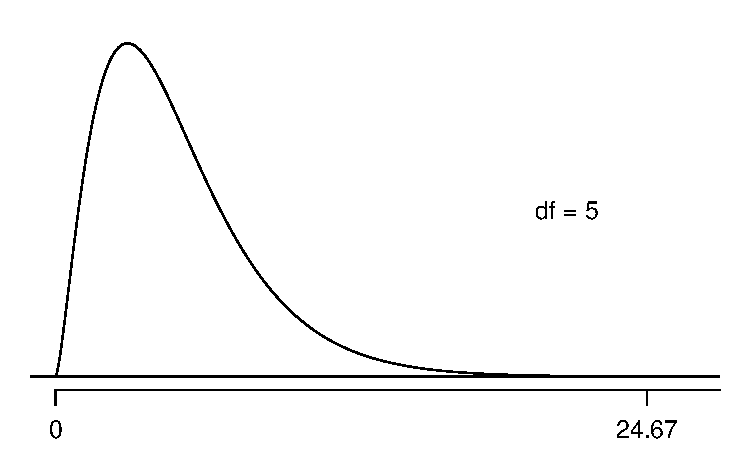
\includegraphics[width=0.67\textwidth]{6-3_chisq_gof/above24Point67WithDF5.pdf}
\end{center}
}
{
p-valor = $P(\chi^2_{df = 5} > 24.67)$\\ é menos do que 0.001
}
\end{frame}
%%%%%%%%%%%%%%%%%%%%%%%%%%%%%%%%%%%

\begin{frame}
\frametitle{Encontrar o p-valor de um teste do qui-quadrado}

\begin{center}
{\scalefont{0.7}
\begin{tabular}{r | rrrr | rrrr r}
  \hline
Cauda superior & 0.3 & 0.2 & 0.1 & 0.05 & 0.02 & 0.01 & 0.005 & 0.001 & \orange{$\rightarrow$}  \\ 
  \hline
df \hfill 1 &  1.07 &  1.64 &  2.71 &  3.84 &  5.41 &  6.63 &  7.88 &  10.83 \\ 
  2 &  2.41 &  3.22 &  4.61 &  5.99 &  7.82 &  9.21 &  10.60 &  13.82 \\ 
  3 &  3.66 &  4.64 &  6.25 &  7.81 &  9.84 &  11.34 &  12.84 &  16.27 \\ 
  4 &  4.88 &  5.99 &  7.78 &  9.49 &  11.67 &  13.28 &  14.86 &  18.47 \\ 
  \rowcolor[gray]{.6}
  5 &  6.06 &  7.29 &  9.24 &  11.07 &  13.39 &  15.09 &  16.75 &  20.52 &\orange{$\rightarrow$} \\ 
  \hline
\end{tabular}
}
\end{center}

\end{frame}

%%%%%%%%%%%%%%%%%%%%%%%%%%%%%%%%%%%

\begin{frame}
\frametitle{Conclusão do teste de hipóteses}
\justifying
\pq{Calculamos um p-valor menor que 0.001. Ao nível de significância de 5\%, qual é a conclusão do teste de hipótese?}

\begin{enumerate}[(a)]
\justifying
\item Rejeitar $H_0$, os dados fornecem evidências convincentes de que os dados são honestos.
\justifying
\solnMult{Rejeitar $H_0$, os dados fornecem evidências convincentes de que os dados são tendenciosos.}
\justifying
\item Não rejeitar $H_0$, os dados fornecem evidências convincentes de que os dados são honestos.
\justifying
\item Não rejeitar $H_0$, os dados fornecem evidências convincentes de que os dados são tendenciosos.
\end{enumerate}

\end{frame}

%%%%%%%%%%%%%%%%%%%%%%%%%%%%%%%%%%%

\begin{frame}
\frametitle{Acontece que...}

\begin{itemize}
\justifying
\item O eixo 1-6 é consistentemente mais curto que os outros dois (2-5 e 3-4), suportando assim a hipótese de que as faces com 1 e 6 são maiores que as outras faces.
\justifying
\item A alegação de Pearson de que 5s e 6s aparecem com mais frequência devido aos pips esculpidos não é suportada por esses dados.
\justifying
\item Os dados usados nos cassinos têm faces niveladas, onde os pontos são preenchidos com um plástico da mesma densidade do material circundante e são precisamente balanceados.

\end{itemize}

\begin{center}
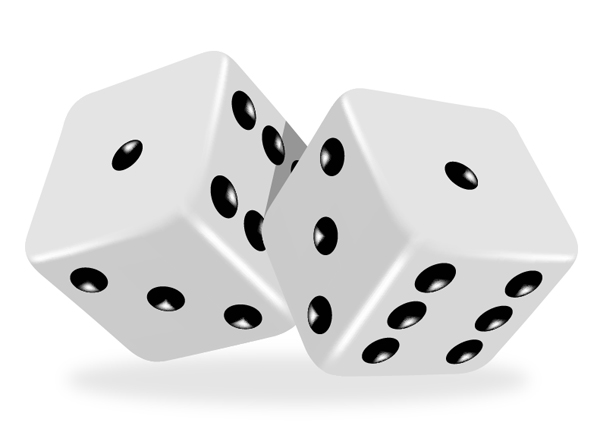
\includegraphics[width=0.3\textwidth]{6-3_chisq_gof/regular.jpeg}
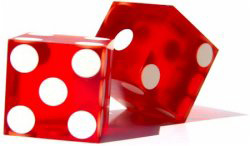
\includegraphics[width=0.3\textwidth]{6-3_chisq_gof/casino.jpeg}
\end{center}


\end{frame}

%%%%%%%%%%%%%%%%%%%%%%%%%%%%%%%%%%%

\begin{frame}
\frametitle{Recapitulando: p-valor do teste qui-quadrado}

\begin{itemize}
\justifying
\item O p-valor do teste qui-quadrado é definido como a área de cauda \hl{acima} da estatística de teste calculada.
\justifying
\item Isso ocorre porque a estatística de teste é sempre positiva e uma estatística de teste mais alta significa um desvio maior da hipótese nula.

\end{itemize}

\begin{center}
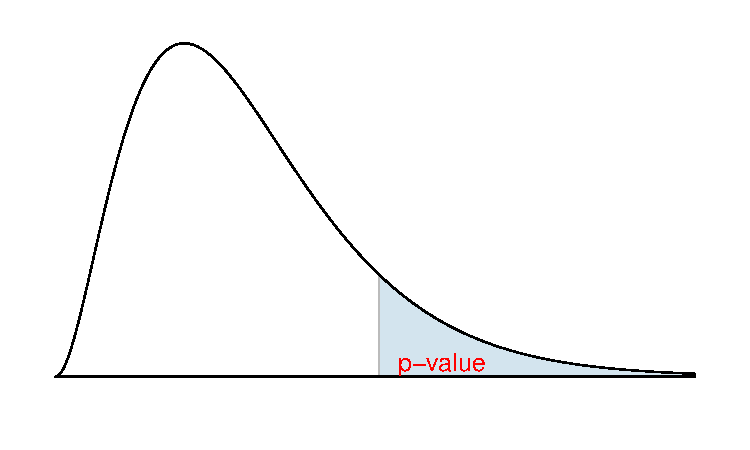
\includegraphics[width=0.7\textwidth]{6-3_chisq_gof/genericChiSquare.pdf}
\end{center}

\end{frame}

%%%%%%%%%%%%%%%%%%%%%%%%%%%%%%%%%%%

\begin{frame}
\frametitle{Condições para o teste do qui-quadrado}

\begin{enumerate}
\justifying
\item \hlGr{Independência:} Cada caso que contribui com uma contagem para a tabela deve ser independente de todos os outros casos na tabela.

\pause
\justifying
\item \hlGr{Tamanho da amostra:} Cada cenário específico (ou seja, cada célula) deve ter pelo menos 5 casos \orange{esperados}.

\pause
\justifying
\item \hlGr{df $>$ 1:} Graus de liberdade devem ser maiores que 1.

\end{enumerate}

\pause
\justifying
Deixar de verificar as condições pode afetar as taxas de erro do teste.

\end{frame}

%%%%%%%%%%%%%%%%%%%%%%%%%%%%%%%%%%%

\subsection{Eleição de 2009 Irã}

%%%%%%%%%%%%%%%%%%%%%%%%%%%%%%%%%%%

\begin{frame}
\frametitle{Eleição de 2009 no Irã}
\justifying
\dq{Falou-se muito sobre fraude eleitoral nas eleições de 2009 no Irã. Vamos comparar os dados de uma pesquisa realizada antes da eleição (dados observados) com os votos informados na eleição para ver se os dois seguem a mesma distribuição.}

\begin{center}
\begin{tabular}{l | r r}
					& \footnotesize{\# observado de} & \footnotesize{\% relatada de} \\
\footnotesize{Candidato}	& \footnotesize{votos na pesquisa} & \footnotesize{votos na eleição} \\
\hline
(1) Ahmedinajad	& 338	& 63.29\% \\
(2) Mousavi		& 136	& 34.10\% \\
(3) Candidatos menores	& 30	& 2.61\% \\
\hline
Total			& 504	& 100\% \\
\pause
			& \hl{$\downarrow$}	& \hl{$\downarrow$}	\\
			& \hl{observado}	& \hl{esperado} \\
			& 			& \hl{distribuição} 	
\end{tabular}
\end{center}

\end{frame}

%%%%%%%%%%%%%%%%%%%%%%%%%%%%%%%%%%%

\begin{frame}
\frametitle{Hipóteses}
\justifying
\dq{Quais são as hipóteses para testar se as distribuições de votos informados e observados são diferentes?}

\soln{
\only<2>{
\begin{itemize}
\justifying
\item[$H_0$:] As contagens observadas da pesquisa seguem a mesma distribuição dos votos relatados.
\justifying
\item[$H_A$:] As contagens observadas da pesquisa não seguem a mesma distribuição que os votos relatados.
\end{itemize}
}}

\end{frame}

%%%%%%%%%%%%%%%%%%%%%%%%%%%%%%%%%%%

\begin{frame}
\frametitle{Cálculo da estatística de teste}


\begin{center}
\scalefont{0.7}
\begin{tabular}{l | r r r}
					& \# observado de & \% relatada de	& \# esperado de \\
Candidato	& votos na pesquisa & votos na eleição		&  votos na pesquisa \\
\hline
(1) Ahmedinajad	& 338	& 63.29\% 	& 504 $\times$ 0.6329 = 319 \\
(2) Mousavi		& 136	& 34.10\%		& 504 $\times$ 0.3410 = 172 \\
(3) Candidatos menores	& 30	& 2.61\% 		& 504 $\times$ 0.0261 = 13\\
\hline
Total			& 504	& 100\%		& 504
\end{tabular}
\end{center}


\pause

\begin{eqnarray*}
\frac{(O_1 - E_1)^2}{E_1} = \frac{(338 - 319)^2}{319} &=& 1.13 \\
\pause
\frac{(O_2 - E_2)^2}{E_2} = \frac{(136 - 172)^2}{172} &=& 7.53 \\
\pause
\frac{(O_2 - E_2)^2}{E_2} = \frac{(30 - 13)^2}{13} &=& 22.23 \\
\pause
 \chi^2_{\mathhl{df = 3 - 1 = 2}} &=& 30.89
\end{eqnarray*}


\end{frame}

%%%%%%%%%%%%%%%%%%%%%%%%%%%%%%%%%%%

\begin{frame}
\frametitle{Conclusão}
\justifying
\pq{Com base nesses cálculos, qual é a conclusão do teste de hipóteses?}

\begin{enumerate}[(a)]
\justifying
\solnMult{o p-valor é baixo, $H_0$ é rejeitada. As contagens observadas na pesquisa \underline {não} seguem a mesma distribuição que os votos relatados.}
\justifying
\item o p-valor é alto, $H_0$ não é rejeitada. As contagens observadas na pesquisa seguem a mesma distribuição dos votos relatados.
\justifying
\item o p-valor é baixo, $H_0$ é rejeitada. As contagens observadas na pesquisa seguem a mesma distribuição que os votos relatados.
\justifying
\item o p-valor é baixo, $H_0$ não é rejeitada. As contagens observadas na pesquisa \underline {não} seguem a mesma distribuição que os votos relatados.
\end{enumerate}

\end{frame}